% ======================================================================
% DEFENSE_PRESENTATION.tex
% Autonomous TEC Atmospheric-Water-Harvesting PV-Cleaning Robot
% Rahma El-Hamouly -- REE598 Graduation Project -- 2026-06-13
% Build: pdflatex DEFENSE_PRESENTATION.tex  (x2)
% ======================================================================
\documentclass[aspectratio=169,10pt]{beamer}

% Shared modern NAC theme: palette, accent-rule frame titles, footline
% progress bar, section dividers, fonts, and all shared packages +
% siunitx units. Build twice with pdflatex for the progress bar.
% ======================================================================
% nac_beamer_theme.tex  --  shared modern Beamer styling for the
% TEC PV-cleaning-robot decks (defense + technical recording).
% pdflatex-safe: no external fonts, no metropolis dependency.
% Build each deck with: pdflatex <deck>.tex  (run twice for the
% progress bar and section references).
% ======================================================================

\usetheme{default}
\useinnertheme{rectangles}
\setbeamertemplate{navigation symbols}{}
\setbeamercovered{transparent}

% --- packages (shared by both decks) ---
\usepackage[utf8]{inputenc}
\usepackage[T1]{fontenc}
\usepackage{lmodern}
\usepackage{xcolor}
\usepackage{tikz}
\usetikzlibrary{calc}
\usepackage{siunitx}
\usepackage{graphicx}
\usepackage{booktabs}
\usepackage{amsmath}

% --- siunitx custom units (shared) ---
\DeclareSIUnit{\Wp}{Wp}
\DeclareSIUnit{\kWp}{kWp}
\DeclareSIUnit{\Wh}{Wh}
\DeclareSIUnit{\kWh}{kWh}
\DeclareSIUnit{\EGP}{EGP}
\DeclareSIUnit{\year}{yr}
\sisetup{detect-weight=true,detect-family=true}

% --- palette (NAC navy / water teal / solar sand) ---
\definecolor{nacblue}{RGB}{20,52,84}
\definecolor{nacblueL}{RGB}{37,86,128}
\definecolor{nacteal}{RGB}{0,150,158}
\definecolor{nacsand}{RGB}{226,170,74}
\definecolor{nacink}{RGB}{31,36,42}
\definecolor{nacgray}{RGB}{108,118,128}
\definecolor{naclight}{RGB}{244,247,250}

% --- base colours ---
\setbeamercolor{normal text}{fg=nacink,bg=white}
\setbeamercolor{alerted text}{fg=nacteal}
\setbeamercolor{structure}{fg=nacblue}
\setbeamercolor{title}{fg=nacblue}
\setbeamercolor{frametitle}{fg=nacblue,bg=white}
\setbeamercolor{itemize item}{fg=nacteal}
\setbeamercolor{itemize subitem}{fg=nacsand}
\setbeamercolor{itemize subsubitem}{fg=nacblueL}
\setbeamercolor{enumerate item}{fg=nacblue}
\setbeamercolor{block title}{fg=white,bg=nacblue}
\setbeamercolor{block body}{fg=nacink,bg=naclight}
\setbeamercolor{caption name}{fg=nacgray}

% --- fonts ---
\setbeamerfont{title}{series=\bfseries,size=\LARGE}
\setbeamerfont{frametitle}{series=\bfseries,size=\large}
\setbeamerfont{block title}{series=\bfseries,size=\normalsize}
\setbeamerfont{author in head/foot}{size=\scriptsize}
\setbeamerfont{title in head/foot}{size=\scriptsize}
\setbeamerfont{date in head/foot}{size=\scriptsize}

% --- blocks: flat, rounded, no shadow ---
\setbeamertemplate{blocks}[rounded][shadow=false]
\setbeamertemplate{itemize items}[circle]
\setbeamertemplate{caption}[numbered]
\setbeamertemplate{frametitle continuation}{}
\setlength{\leftmargini}{1.4em}

% --- frame title with a teal accent rule underneath ---
\setbeamertemplate{frametitle}{%
  \nointerlineskip%
  \vskip0.55em%
  \begin{beamercolorbox}[wd=\paperwidth,sep=0pt,leftskip=0.55cm,rightskip=0.55cm]{frametitle}%
    {\usebeamerfont{frametitle}\usebeamercolor[fg]{frametitle}\insertframetitle\strut\par}%
    \vskip3pt%
    {\color{nacteal}\rule{2.4cm}{2.2pt}}%
  \end{beamercolorbox}%
  \vskip0.35em%
}

% --- minimal footline with a teal progress bar ---
\setbeamertemplate{footline}{%
  \pgfmathsetmacro{\nacprog}{\insertframenumber/(\inserttotalframenumber<1?1:\inserttotalframenumber)}%
  \hbox to\paperwidth{%
    \rlap{\color{nacblue!12}\rule{\paperwidth}{1.6pt}}%
    \rlap{\color{nacteal}\rule{\nacprog\paperwidth}{1.6pt}}\hfil}%
  \vskip2pt%
  \hbox to\paperwidth{%
    \hskip0.45cm{\color{nacgray}\usebeamerfont{author in head/foot}\insertshortauthor}\hfil
    {\color{nacgray}\usebeamerfont{title in head/foot}\insertshorttitle}\hfil
    {\color{nacblue}\usebeamerfont{date in head/foot}\insertframenumber\,/\,\inserttotalframenumber}\hskip0.45cm}%
  \vskip3pt%
}

% --- section divider slides ---
\AtBeginSection[]{%
  {\setbeamertemplate{footline}{}%
   \begin{frame}[plain,noframenumbering]%
    \begin{tikzpicture}[remember picture,overlay]%
      \fill[nacblue](current page.south west)rectangle(current page.north east);%
      \fill[nacteal](current page.south west)rectangle([yshift=6pt]current page.south east);%
    \end{tikzpicture}%
    \vfill
    \begin{center}
      {\color{nacsand}\large\bfseries Part~\insertsectionnumber}\\[0.55em]
      {\color{white}\Huge\bfseries\insertsection}\\[0.75em]
      {\color{nacteal}\rule{3cm}{2.5pt}}
    \end{center}
    \vfill
   \end{frame}}%
}

% --- reusable custom title slide: \nactitleframe ---
\newcommand{\nactitleframe}[5]{%
  % #1 eyebrow line, #2 title (may use \\), #3 subtitle, #4 author, #5 footer line
  {\setbeamertemplate{footline}{}%
   \begin{frame}[plain,noframenumbering]%
    \begin{tikzpicture}[remember picture,overlay]%
      \fill[nacblue](current page.south west)rectangle(current page.north east);%
      \fill[nacteal](current page.south west)rectangle([yshift=7pt]current page.south east);%
    \end{tikzpicture}%
    \vfill
    \begin{center}
      {\color{nacsand}\large\bfseries #1}\\[1.05em]
      {\color{white}\usebeamerfont{title}#2}\\[0.8em]
      {\color{nacteal}\rule{4cm}{2.5pt}}\\[0.8em]
      {\color{white!88}\large #3}\\[1.7em]
      {\color{white}\large\bfseries #4}\\[0.35em]
      {\color{white!75}\normalsize #5}
    \end{center}
    \vfill
   \end{frame}}%
}


% Graphics path
\graphicspath{{figures/}{figures/slides/}}

% --- Title metadata ---
\title[Self-Watering PV-Cleaning Robot]{Autonomous Thermoelectric Water-Harvesting\\Robot for Cleaning Rooftop PV in Egypt}
\subtitle{A self-watering, rail-guided cleaner for the New Administrative Capital}
\author[R. El-Hamouly]{Rahma El-Hamouly}
\institute[REE598]{Graduation Project REE598 \\ Faculty of Engineering}
\date{13 June 2026}

% Footline-safe short institute already set above

\begin{document}

% ===================== 1. TITLE =====================
\nactitleframe
  {Graduation Project {\textbullet} REE\,598 {\textbullet} Thesis Defense}
  {\bfseries Autonomous Thermoelectric Water-Harvesting\\[0.15em]Robot for Cleaning Rooftop PV in Egypt}
  {A self-watering, rail-guided cleaner for the New Administrative Capital}
  {Rahma El-Hamouly}
  {Faculty of Engineering \quad{\textbullet}\quad 13 June 2026}

% ===================== 2. OUTLINE =====================
\begin{frame}{Outline}
  \begin{columns}[T]
    \begin{column}{0.5\textwidth}
      \begin{enumerate}\setlength\itemsep{0.35em}
        \item Motivation and problem
        \item Objectives
        \item Background and the gap
        \item Why TEC: feasibility evidence
        \item Site and climate: NAC
        \item System architecture
      \end{enumerate}
    \end{column}
    \begin{column}{0.5\textwidth}
      \begin{enumerate}\setlength\itemsep{0.35em}\setcounter{enumi}{6}
        \item Water harvester and sizing
        \item Robot: crawler to rail-guided
        \item Control and autonomy
        \item Simulation results
        \item Prototype, economics, contributions
        \item Limitations and conclusion
      \end{enumerate}
    \end{column}
  \end{columns}
\end{frame}

\section{Problem \& Motivation}
% ===================== 3. MOTIVATION =====================
\begin{frame}{Motivation: dust costs power, and water is scarce}
  \begin{itemize}\setlength\itemsep{0.5em}
    \item Egypt is building solar-powered desert cities: NAC, New Alamein, New Mansoura.
    \item Dust on PV glass in arid Egypt cuts output \SI{0.3}{} to \SI{0.8}{\percent} per day. A panel left a month can lose a fifth of its yield.
    \item Wet cleaning recovers it, but clean water in the desert means trucking, and trucking is the recurring cost that kills the economics.
    \item So the resource that fixes the soiling problem is the one the desert does not have.
  \end{itemize}
  \vspace{0.4em}
  \begin{block}{The idea}
    Make the cleaner produce its own water, by condensing it out of the night air.
  \end{block}
\end{frame}

% ===================== 4. PROBLEM + OBJECTIVES =====================
\begin{frame}{Problem statement and objectives}
  \textbf{Problem.} Keep rooftop PV clean in an arid climate without a water supply chain and without a person on the roof.
  \vspace{0.6em}

  \textbf{Objectives.}
  \begin{enumerate}\setlength\itemsep{0.4em}
    \item Show thermoelectric (TEC) water harvesting actually yields water in Egyptian desert air.
    \item Size a dockside harvester for a real residential array in the NAC.
    \item Design an autonomous robot that cleans a tilted panel and refills from that water.
    \item Validate the motion in simulation and prove the core physics on a cheap bench.
  \end{enumerate}
\end{frame}

\section{Background \& Feasibility}
% ===================== 5. BACKGROUND / RELATED WORK =====================
\begin{frame}{Background and the gap}
  \begin{columns}[T]
    \begin{column}{0.52\textwidth}
      \textbf{PV cleaning robots}
      \begin{itemize}\small
        \item Rail-guided wipers (e.g.\ Ecoppia E4) are proven at utility scale, but dry-brush only.
        \item Wet cleaning needs a water feed, which is exactly the desert bottleneck.
      \end{itemize}
      \vspace{0.5em}
      \textbf{Atmospheric water harvesting}
      \begin{itemize}\small
        \item Sorption: high yield, slow, bulky desiccant.
        \item Vapour-compression (VCR): efficient at scale, refrigerant and compressor.
        \item Thermoelectric (TEC): solid-state, silent, modular, no moving parts.
      \end{itemize}
    \end{column}
    \begin{column}{0.46\textwidth}
      \begin{block}{The gap}
        Cleaning robots assume a water supply. Water harvesters are standalone appliances. Nobody puts the two together.
      \end{block}
      \vspace{0.4em}
      \begin{block}{This work}
        A PV cleaner that harvests its own distilled water on site. TEC chosen for its modularity at rooftop scale.
      \end{block}
    \end{column}
  \end{columns}
\end{frame}

% ===================== 6. FEASIBILITY EVIDENCE / WHY TEC =====================
\begin{frame}{Feasibility evidence: does TEC harvesting even work here?}
  Validated first against Benban (Aswan), the worst-case arid reference, using \num{8784} hourly climate records.
  \vspace{0.4em}
  \begin{itemize}\setlength\itemsep{0.35em}
    \item Egyptian-market TEC1-12706 module, \SI{130}{\EGP} ($\approx$\,\SI{2.71}{} USD).
    \item Extracted coefficients: $\alpha=\SI{0.0513}{\volt\per\kelvin}$, $R=\SI{2.00}{\ohm}$, $K=\SI{0.546}{\watt\per\kelvin}$.
    \item A night-only smart strategy with a \SI{5}{\kelvin} condensation margin yields measurable water every modelled month.
  \end{itemize}
  \vspace{0.3em}
  \begin{block}{Why TEC over VCR at this scale}
    Solid-state, no refrigerant, fully modular: add or drop tiles to resize the harvester. The penalty is efficiency, which sets up the honest sizing trade later.
  \end{block}
\end{frame}

% ===================== 7. SITE + CLIMATE (figure) =====================
\begin{frame}{Site selection: the New Administrative Capital}
  \begin{columns}[T]
    \begin{column}{0.5\textwidth}
      \begin{itemize}\setlength\itemsep{0.4em}
        \item Reference deployment moved from Benban to a NAC rooftop (\ang{30.03} N, \ang{31.73} E).
        \item Re-ran the same engine on NASA POWER hourly data for 2025.
        \item Per-tile yield rises from \SI{5.35}{\liter\per\year} (Benban) to \SI{38.7}{\liter\per\year} (NAC).
        \item Factor \textbf{7.2}, mean COP \textbf{1.91}, and no dead summer month.
      \end{itemize}
      \vspace{0.3em}
      \begin{block}{Takeaway}
        Cooler, more humid coastal-influenced air at the NAC makes harvesting far more productive than the Aswan desert.
      \end{block}
    \end{column}
    \begin{column}{0.5\textwidth}
      \centering
      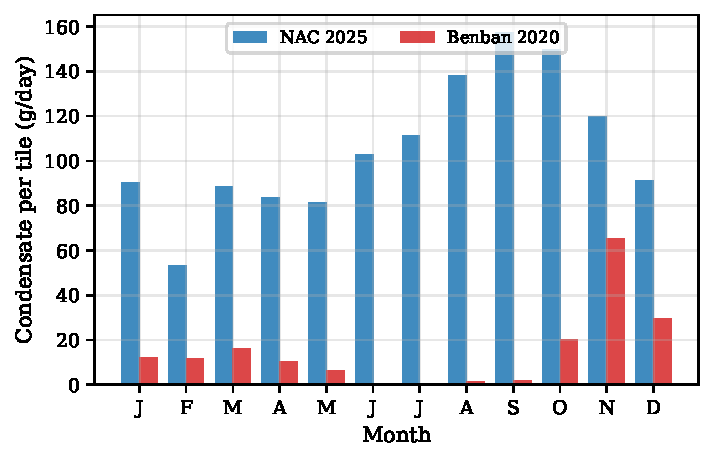
\includegraphics[width=\linewidth]{nac_monthly_water.pdf}\\
      {\scriptsize NAC monthly per-tile water yield, 2025.}
    \end{column}
  \end{columns}
\end{frame}

\section{System Design}
% ===================== 8. SYSTEM ARCHITECTURE (figure) =====================
\begin{frame}{System architecture: three scales, one design}
  \begin{columns}[T]
    \begin{column}{0.46\textwidth}
      \textbf{Target scales}
      \begin{itemize}\small\setlength\itemsep{0.3em}
        \item Commercial rooftops (50--500 kWp)
        \item \textbf{Residential rooftops} (reference case)
        \item Street-lamp PV (single panel)
      \end{itemize}
      \vspace{0.4em}
      \textbf{Subsystems}
      \begin{itemize}\small\setlength\itemsep{0.3em}
        \item Dockside TEC water generator
        \item Distilled tank, pump, filter
        \item Rail-guided cleaning carriage
        \item PV, MPPT, battery
        \item Two-tier ROS 2 controller
      \end{itemize}
    \end{column}
    \begin{column}{0.52\textwidth}
      \centering
      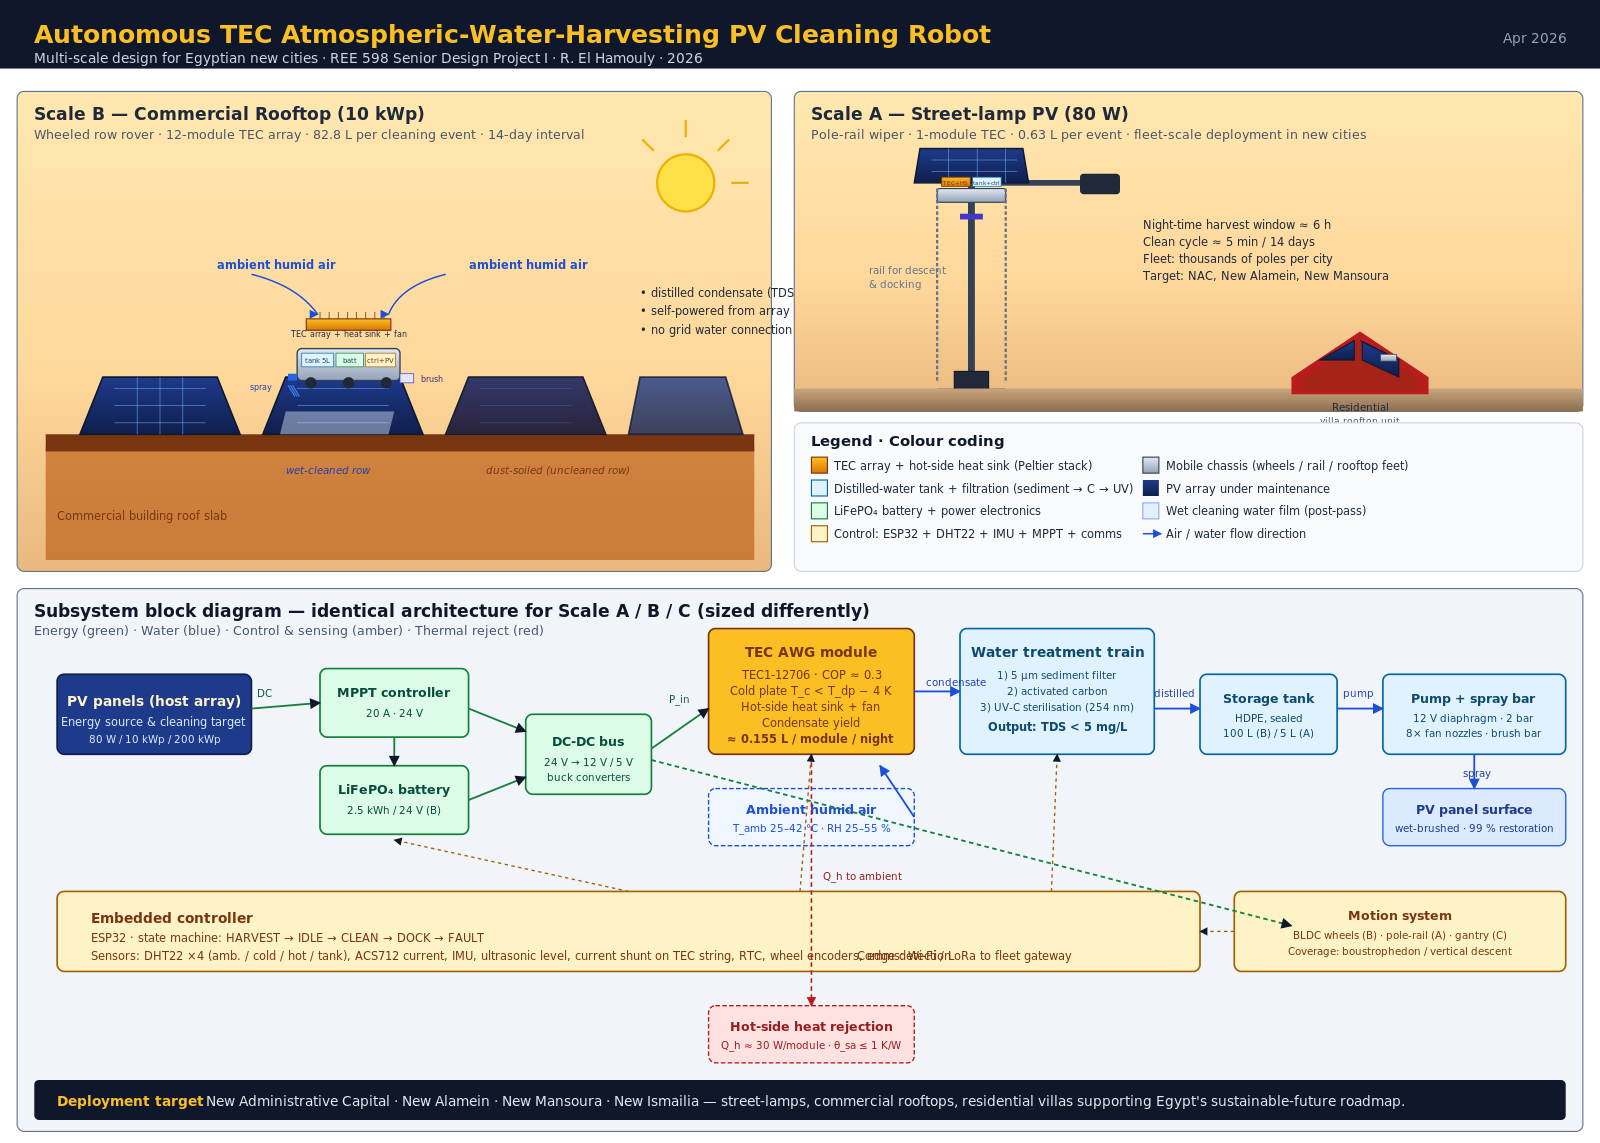
\includegraphics[width=\linewidth]{system_architecture.png}\\
      {\scriptsize Subsystem block diagram.}
    \end{column}
  \end{columns}
\end{frame}

% ===================== 9. TEC AWG DESIGN (figure) =====================
\begin{frame}{TEC water generator: how a tile makes water}
  \begin{columns}[T]
    \begin{column}{0.5\textwidth}
      \begin{itemize}\setlength\itemsep{0.35em}
        \item Peltier tile chills a cold plate below the dew point. Moisture condenses; drops are collected.
        \item Coupled heat-and-mass-transfer solver finds the operating point per hour of climate.
        \item At the NAC: \SI{38.7}{\liter\per\year} per tile, \SI{106}{\gram\per\day}, mean COP 1.91.
        \item Specific energy \SI{1.45}{\kWh\per\liter} thermoelectric.
      \end{itemize}
    \end{column}
    \begin{column}{0.5\textwidth}
      \centering
      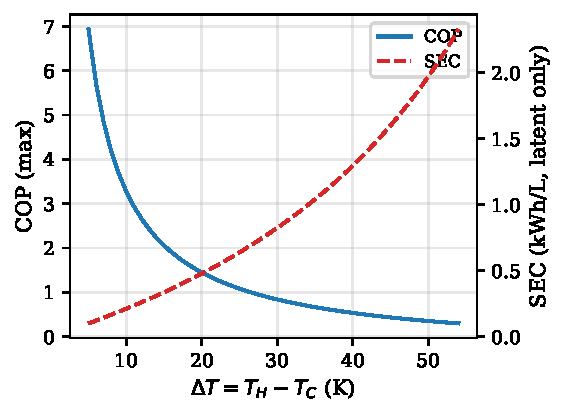
\includegraphics[width=\linewidth]{fig_cop_sec_dT.pdf}\\
      {\scriptsize COP and specific energy versus cold-side $\Delta T$.}
    \end{column}
  \end{columns}
\end{frame}

% ===================== 10. SIZING: honest trade =====================
\begin{frame}{Sizing the dock: the honest self-supply trade}
  The microfibre brush cleans at \SI{0.3}{\liter\per\square\meter}, so washing \SI{46}{\square\meter} of glass every \SI{3.5}{} days needs only \SI{1.44}{} m$^3$/year. Full atmospheric self-supply is feasible: \textbf{38 tiles} at \SI{6.47}{\kWh\per\day}, about \SI{14}{\percent} of what the array generates.
  \vspace{0.5em}
  \begin{center}
  \begin{tabular}{lccc}
    \toprule
    Self-supply fraction & 25\,\% & 50\,\% & 100\,\% \\
    \midrule
    TEC tiles            & 10 & 19 & \textbf{38} \\
    Energy (kWh/day)     & 1.75 & 3.25 & \textbf{6.47} \\
    Dock cost (EGP)      & 85{,}320 & 137{,}253 & \textbf{224{,}756} \\
    \bottomrule
  \end{tabular}
  \end{center}
  \vspace{0.4em}
  \begin{block}{Selected design}
    100\,\% self-supply: 38 tiles at the 3.5-day schedule (or 19 tiles weekly). Standalone cost is dominated by the dock's own PV and battery; drawing from the house \SI{9.9}{\kWp} array, the marginal AWG hardware is about \SI{14000}{} EGP.
  \end{block}
\end{frame}

% ===================== 11. ENERGY & POWER BUDGET (figure) =====================
\begin{frame}{Energy and power budget}
  \begin{columns}[T]
    \begin{column}{0.5\textwidth}
      \begin{itemize}\setlength\itemsep{0.35em}
        \item Selected 38-tile dock draws \SI{6.47}{\kWh\per\day}.
        \item TEC tiles dominate; fans are the next largest draw; cleaning and the controller are negligible.
        \item Supplied by dedicated PV plus a battery buffer so harvesting can run on cool night air.
        \item Cleaning a panel costs about \SI{74}{\Wh} per event, a rounding error against the harvester.
      \end{itemize}
    \end{column}
    \begin{column}{0.5\textwidth}
      \centering
      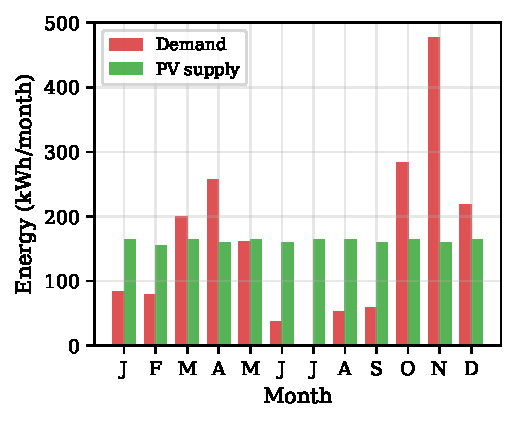
\includegraphics[width=\linewidth]{fig_energy_balance.pdf}\\
      {\scriptsize Daily energy balance by subsystem.}
    \end{column}
  \end{columns}
\end{frame}

% ===================== 12. ROBOT MECH + EVOLUTION (3D figure) =====================
\begin{frame}{Robot mechanical design: from crawler to rail}
  \begin{columns}[T]
    \begin{column}{0.5\textwidth}
      \textbf{Why the design changed.} The first concept was a free differential-drive crawler. In simulation it could not yaw on \ang{24} glass: the wheels broke traction and it slid down the fall line.
      \vspace{0.5em}

      \textbf{The fix.} A rail-guided carriage. Two rails carry an \SI{8}{kg} carriage with a full-width \SI{0.96}{m} brush. It only ever moves along the fall line, so steering on glass is no longer needed.
    \end{column}
    \begin{column}{0.5\textwidth}
      \centering
      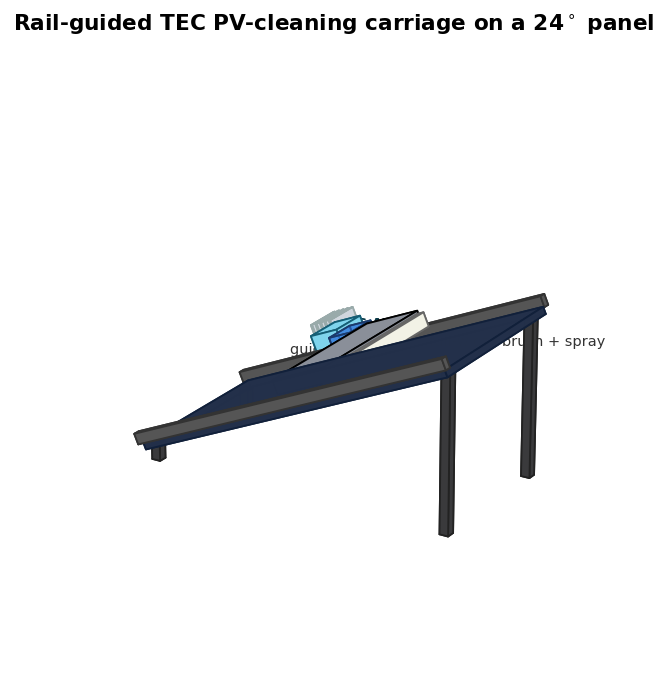
\includegraphics[width=\linewidth]{robot_3d.png}\\
      {\scriptsize Rail-guided cleaning carriage, isometric view.}
    \end{column}
  \end{columns}
\end{frame}

% ===================== 13. CAD / DRIVE DETAIL =====================
\begin{frame}{Drive train: full-width brush, rack and pinion}
  \begin{columns}[T]
    \begin{column}{0.55\textwidth}
      \begin{itemize}\setlength\itemsep{0.35em}
        \item Full-width brush cleans the whole panel in one pass, so no side-to-side weaving.
        \item Rack-and-pinion drive on both rails: positive grip, no slip on the tilt.
        \item Required torque $\geq$ \SI{0.84}{\newton\meter} at a \SI{30}{mm} pinion, about \SI{38}{rpm}.
        \item Coverage: \SI{66.7}{s} per panel (down and up) against \SI{230}{s} for the old boustrophedon path.
        \item Water use \SI{3.6}{\liter} per cleaning event.
      \end{itemize}
    \end{column}
    \begin{column}{0.45\textwidth}
      \begin{block}{Geometry}
        Carriage \SI{8}{kg}; brush \SI{0.96}{m}; two \SI{2.4}{m} rails; total rack \SI{4.8}{m}; cleaning speed \SI{0.06}{\meter\per\second}.
      \end{block}
      \begin{block}{Why it is faster}
        One full-width sweep replaces six narrow passes, so a panel is clean in about a quarter of the time.
      \end{block}
    \end{column}
  \end{columns}
\end{frame}

% ===================== 14. CONTROL & AUTONOMY =====================
\begin{frame}{Control and autonomy: two-tier ROS 2}
  \begin{columns}[T]
    \begin{column}{0.52\textwidth}
      \textbf{Why two tiers}
      \begin{itemize}\small\setlength\itemsep{0.3em}
        \item Raspberry Pi 4 runs ROS 2 Humble: supervisor, planning, logging.
        \item ESP32 with micro-ROS handles hard real-time PWM, encoders, and PID.
        \item One MCU cannot do both soft planning and tight motor loops reliably.
      \end{itemize}
      \vspace{0.3em}
      \textbf{No SLAM}
      \begin{itemize}\small\setlength\itemsep{0.3em}
        \item Dead reckoning along the rails, plus edge re-registration at panel ends. The rail removes the need for a map.
      \end{itemize}
    \end{column}
    \begin{column}{0.48\textwidth}
      \begin{block}{Supervisor FSM}
        \centering
        Idle $\rightarrow$ Harvest $\rightarrow$ Store $\rightarrow$ Clean $\rightarrow$ Dock
      \end{block}
      \begin{itemize}\small\setlength\itemsep{0.3em}
        \item Harvest and store run at night; clean runs on the 3.5-day interval.
        \item Sweep coverage: descend the fall line, then climb back.
        \item Safety layers gate motion on tank level and rail limits.
      \end{itemize}
    \end{column}
  \end{columns}
\end{frame}

\section{Results \& Validation}
% ===================== 15. SIMULATION SETUP + KEY RESULT =====================
\begin{frame}{Simulation: the result that drove the design}
  \begin{columns}[T]
    \begin{column}{0.52\textwidth}
      \textbf{Setup}
      \begin{itemize}\small\setlength\itemsep{0.3em}
        \item Gazebo Classic 11 with ROS 2 Humble, run headless.
        \item Robot URDF on a \ang{24} tilted panel with rails.
      \end{itemize}
      \vspace{0.4em}
      \textbf{Key engineering result}
      \begin{itemize}\small\setlength\itemsep{0.3em}
        \item The free crawler could not turn on the tilt: it lost traction and slid. Infeasible.
        \item Switching to a rail-guided carriage removed the steering problem entirely.
        \item This is why the final design is rail-guided, not free-roaming.
      \end{itemize}
    \end{column}
    \begin{column}{0.48\textwidth}
      \centering
      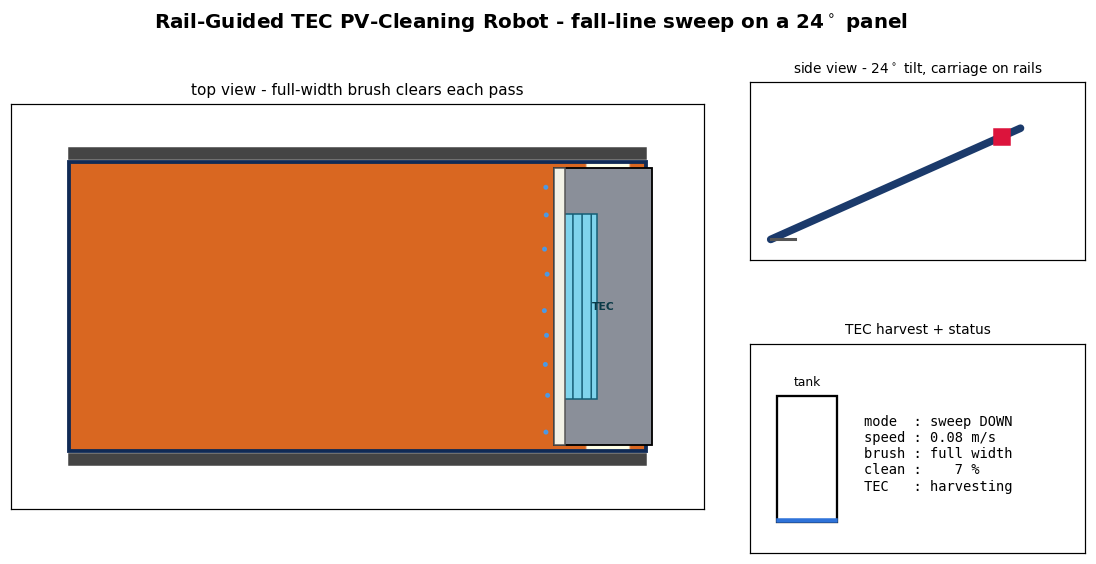
\includegraphics[width=\linewidth]{sim_still_1.png}\\[0.3em]
      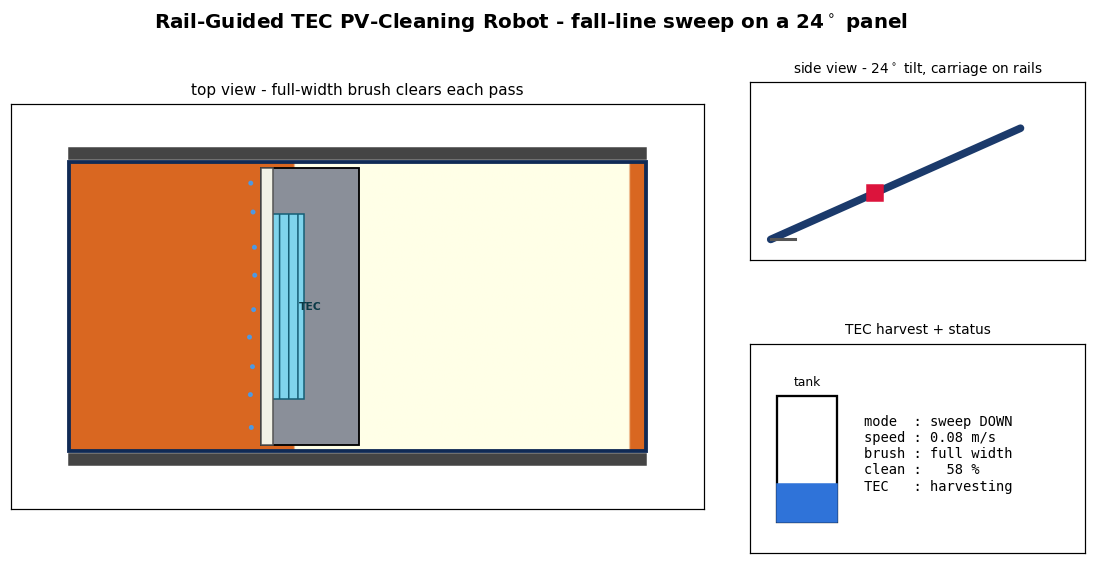
\includegraphics[width=\linewidth]{sim_still_2.png}\\
      {\scriptsize Rail-guided sweep on the \ang{24} panel.}
    \end{column}
  \end{columns}
\end{frame}

% ===================== 16. SIMULATION VALIDATION =====================
\begin{frame}{Simulation: rail-guided sweep validated}
  \begin{columns}[T]
    \begin{column}{0.5\textwidth}
      \begin{itemize}\setlength\itemsep{0.4em}
        \item The carriage descends the fall line and climbs back, completing a full down-and-up sweep.
        \item Lateral drift stays below \SI{1}{mm}: it tracks the rails cleanly.
        \item It stays on the rails through the whole cycle, no derailment.
        \item Confirms the \SI{66.7}{s} per-panel coverage used in the energy budget.
      \end{itemize}
    \end{column}
    \begin{column}{0.5\textwidth}
      \centering
      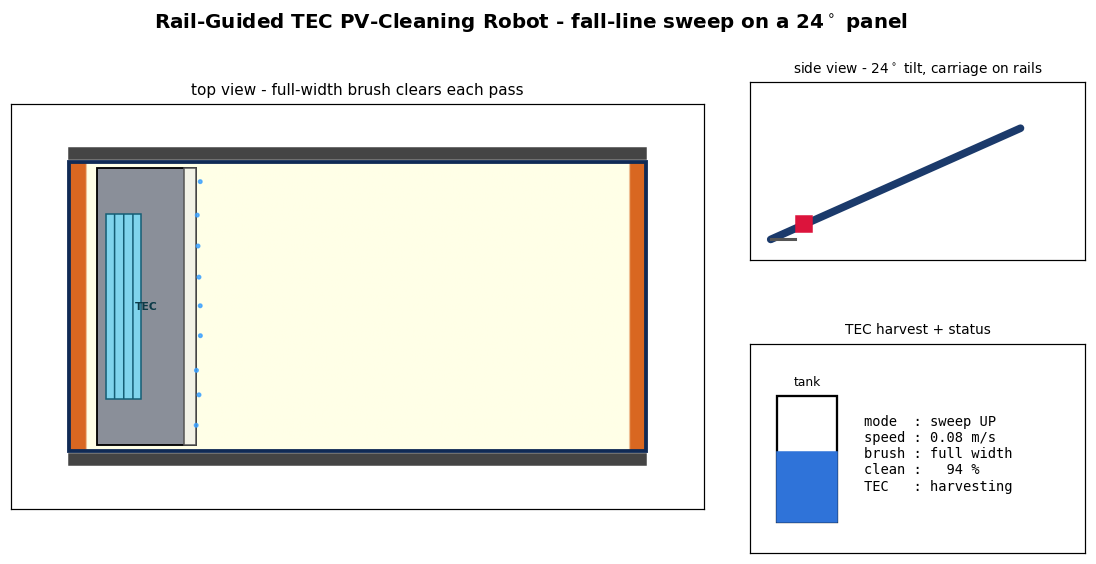
\includegraphics[width=\linewidth]{sim_still_3.png}\\[0.3em]
      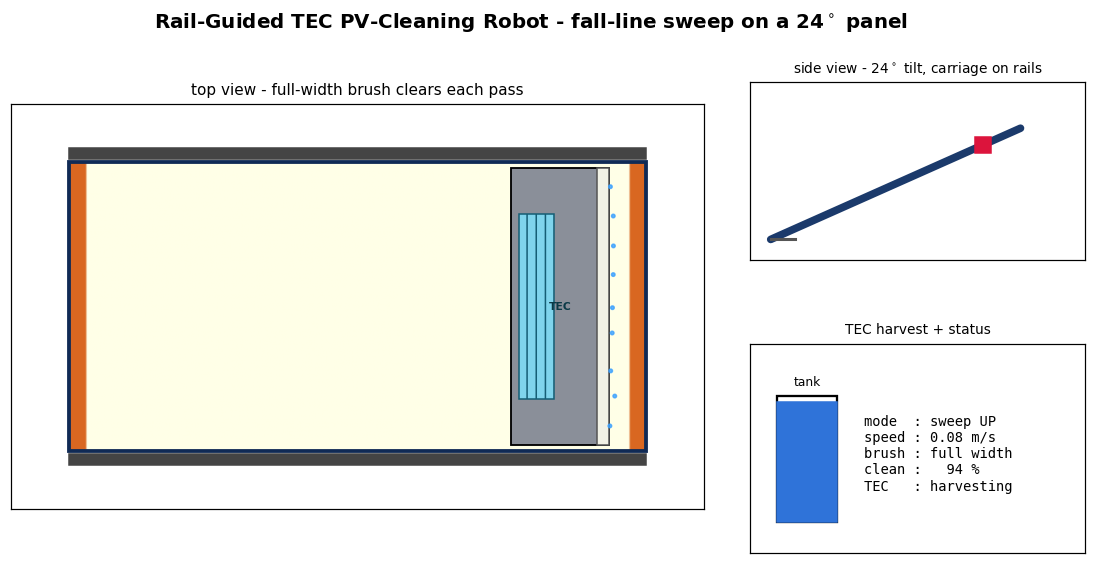
\includegraphics[width=\linewidth]{sim_still_4.png}\\
      {\scriptsize Descent and climb stills from the headless run.}
    \end{column}
  \end{columns}
\end{frame}

% ===================== 17. RESULTS: water yield (figure) =====================
\begin{frame}{Results: annual water yield and monthly profile}
  \begin{columns}[T]
    \begin{column}{0.5\textwidth}
      \begin{itemize}\setlength\itemsep{0.35em}
        \item Per tile at the NAC: \SI{38.7}{\liter\per\year}, \SI{106}{\gram\per\day}.
        \item The 38-tile dock delivers about \SI{3.94}{\liter\per\day}, the full cleaning demand.
        \item Yield holds across all twelve months, with a summer peak and no dead season.
        \item Mean COP 1.91 over \num{3610} operating hours per year.
      \end{itemize}
    \end{column}
    \begin{column}{0.5\textwidth}
      \centering
      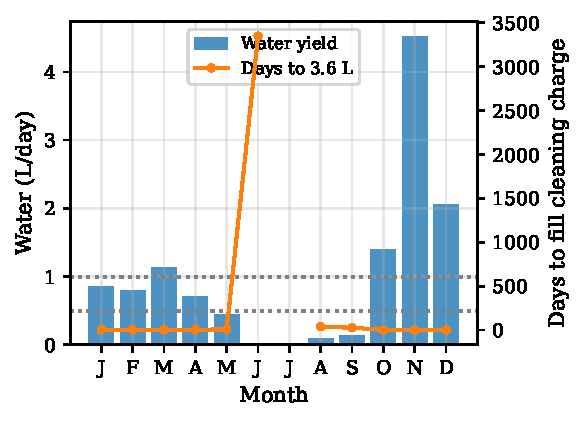
\includegraphics[width=\linewidth]{fig_monthly_water.pdf}\\
      {\scriptsize Monthly water yield across the year.}
    \end{column}
  \end{columns}
\end{frame}

% ===================== 18. FEASIBILITY CONCLUSION =====================
\begin{frame}{Feasibility conclusion: what actually closes}
  \begin{itemize}\setlength\itemsep{0.45em}
    \item One robot per array, not per panel: a shared dock harvests for the whole array rather than a closed loop on each panel.
    \item At the microfibre dose of \SI{0.3}{\liter\per\square\meter}, demand drops to \SI{1.44}{} m$^3$/year, so the dock harvests the full supply on site.
    \item A \SI{300}{\liter} storage tank smooths month-to-month yield so the supply rarely runs dry.
    \item The robot mechanics are unchanged across sites: the \ang{26} NAC tilt adds only \SI{5}{\percent} traction torque, inside the motor band.
  \end{itemize}
  \vspace{0.3em}
  \begin{block}{Honest headline}
    100\,\% self-supply is feasible: 38 tiles at the 3.5-day schedule (19 weekly), about \SI{14}{\percent} of array energy, removing trucked water entirely.
  \end{block}
\end{frame}

\section{Prototype, Economics \& Outcomes}
% ===================== 19. PROTOTYPE + BUYLIST =====================
\begin{frame}{Prototype: proving the physics for 5{,}545 EGP}
  \begin{columns}[T]
    \begin{column}{0.55\textwidth}
      \textbf{Minimum bench} (about \SI{116}{} USD), all buyable in Cairo, no imports.
      \begin{center}\small
      \begin{tabular}{lr}
        \toprule
        Block & EGP \\
        \midrule
        TEC harvesting core (4 tiles) & 2{,}110 \\
        Cleaning head (pump, brush) & 960 \\
        Sensors (DHT22, INA219, DS18B20) & 585 \\
        Control and power & 1{,}890 \\
        \midrule
        \textbf{Total} & \textbf{5{,}545} \\
        \bottomrule
      \end{tabular}
      \end{center}
    \end{column}
    \begin{column}{0.45\textwidth}
      \textbf{What it proves}
      \begin{itemize}\small\setlength\itemsep{0.3em}
        \item Four tiles condense measurable water in NAC-type air, logged.
        \item Pump and brush wet and sweep a soiled glass coupon.
      \end{itemize}
      \vspace{0.4em}
      \textbf{What stays simulated}
      \begin{itemize}\small\setlength\itemsep{0.3em}
        \item Rail-guided motion (proven in Gazebo).
        \item The full dock, PV and battery chain.
      \end{itemize}
      About a quarter of the \SI{22365}{\EGP} full bench.
    \end{column}
  \end{columns}
\end{frame}

% ===================== 20. ECONOMICS =====================
\begin{frame}{Economics: where the money goes}
  \begin{columns}[T]
    \begin{column}{0.52\textwidth}
      \begin{itemize}\setlength\itemsep{0.4em}
        \item A standalone off-grid 38-tile dock prices at about \SI{224756}{\EGP}, dominated by its own dedicated PV and battery.
        \item The house already has a \SI{9.9}{\kWp} array, so the dock draws from it and skips the dedicated supply.
        \item The marginal AWG hardware for 100\,\% self-supply is then about \SI{14000}{\EGP}: tiles, sinks, fans, cold plate, switching.
        \item The cleaning carriage itself is a minor line item.
      \end{itemize}
    \end{column}
    \begin{column}{0.48\textwidth}
      \begin{block}{Cost driver}
        Dedicated off-grid supply dominates the standalone price. Grid-coupled to the house array, 100\,\% self-supply is cheap.
      \end{block}
      \begin{block}{Marginal AWG hardware (grid-coupled)}
        \centering\small
        38 tiles + sinks + fans + cold plate + switching $\approx$ \SI{14}{k} EGP
      \end{block}
    \end{column}
  \end{columns}
\end{frame}

% ===================== 21. CONTRIBUTIONS / NOVELTY =====================
\begin{frame}{Contributions and novelty}
  \begin{enumerate}\setlength\itemsep{0.5em}
    \item A PV cleaner that harvests its own distilled water on site, closing the gap between dry rail robots and standalone water generators.
    \item A validated TEC harvesting model on real Egyptian climate data, with the 7.2$\times$ NAC-versus-Benban yield finding.
    \item An honest self-supply trade: at the microfibre dose, full closure is feasible at 38 tiles, about \SI{14}{\percent} of array energy.
    \item A documented design pivot, crawler to rail-guided, driven by a reproducible simulation result rather than assumption.
    \item A \SI{5545}{\EGP} bench, sourced entirely in Cairo, that proves the core physics.
  \end{enumerate}
\end{frame}

% ===================== 22. LIMITATIONS + FUTURE WORK =====================
\begin{frame}{Limitations and future work}
  \begin{columns}[T]
    \begin{column}{0.5\textwidth}
      \textbf{Limitations}
      \begin{itemize}\small\setlength\itemsep{0.35em}
        \item Full self-supply depends on the \SI{0.3}{\liter\per\square\meter} dose holding in the field; a wetter dose would raise the tile count.
        \item Yield modelled on one climate year; multi-year variability not yet captured.
        \item Rail motion validated in simulation, not yet on physical rails.
        \item Battery cost dominates and depends on a volatile market.
      \end{itemize}
    \end{column}
    \begin{column}{0.5\textwidth}
      \textbf{Future work}
      \begin{itemize}\small\setlength\itemsep{0.35em}
        \item Build the full rail bench and measure real coverage.
        \item Field-log harvester yield across a full year at the NAC.
        \item Hybrid harvesting (radiative pre-cooling) to lift COP.
        \item Extend the design to the commercial and street-lamp scales.
      \end{itemize}
    \end{column}
  \end{columns}
\end{frame}

% ===================== 23. REFERENCES =====================
\begin{frame}{Key references}
  \footnotesize
  \begin{enumerate}\setlength\itemsep{0.4em}
    \item NASA POWER Project. Hourly meteorological data, NAC point (\ang{30.03} N, \ang{31.73} E), 2025.
    \item Ecoppia. Robotic dry-cleaning systems for utility-scale PV. Technical documentation.
    \item TEC1-12706 thermoelectric module datasheet, Egyptian-market supplier.
    \item IEC 61724-1. Photovoltaic system performance monitoring.
    \item Open Robotics. ROS 2 Humble and Gazebo Classic 11 documentation.
    \item J. Kabeel et al. Atmospheric water generation in arid climates: a review.
  \end{enumerate}
\end{frame}

% ===================== 24. CONCLUSION / Q&A =====================
{\setbeamertemplate{footline}{}
\begin{frame}[plain]
  \begin{center}
    {\Large\color{nacblue}\textbf{Conclusion}}\\[0.8em]
  \end{center}
  \begin{itemize}\setlength\itemsep{0.45em}
    \item A rail-guided robot that cleans rooftop PV and refills from water it condenses out of the air.
    \item TEC harvesting works in Egyptian desert air, and the NAC delivers 7.2$\times$ the Benban yield.
    \item Full self-supply is feasible at the microfibre dose: a 38-tile dock, about \SI{14}{\percent} of array energy, is the honest, buildable answer.
    \item The motion is validated in Gazebo and the physics is provable on a \SI{5545}{\EGP} Cairo bench.
  \end{itemize}
  \vspace{0.8em}
  \begin{center}
    {\Large\color{nacteal}\textbf{Thank you. Questions?}}\\[0.4em]
    \small Rahma El-Hamouly \quad|\quad REE598 \quad|\quad 13 June 2026
  \end{center}
\end{frame}}

\end{document}
